%! Author = leona
%! Date = 09/02/24
% !TeX root = ../thesis-main.tex

\chapter{Background}
\label{chap:background}
Presented in this chapter are some core concepts that serve as a knowledge base upon which this thesis is built.
First, we will introduce the reader to the concept of \ac{ac}. Then we will examine ScaFi, a state-of-the-art implementation of \ac{ac}, that inspired this thesis's project.
Finally, we will introduce the Rust programming language, which is the language of choice for the implementation of the project.

\section{Aggregate Programming and Field Calculus}
Aggregate programming \cite{Beal2016} is a programming approach that aims to shift the focus on the individual device perspective that is typical of traditional programming approaches, which
inevitably entangles the system's behavior design with aspects of distributed systems design (such as efficient and reliable communication, coordination and fault tolerance) to an approach that raises
the abstraction level from individual devices to large aggregations of devices. It does so by exploiting the concepts of computational fields and \ac{fc} \cite{10.1145/3285956, 10.1007/978-3-642-45364-9_11}.\\

Within the \ac{fc}, a \textit{computational field} is a function mapping every computational device in a network, represented by a dynamic and reflexive neighboring relationship between devices, to a computational object.
Depending on the computational object in question, there can be many examples of computational fields:
\begin{itemize}
    \item \textbf{Scalar fields}: a field that maps every device to the value of some sensor reading;
    \item \textbf{Vector fields}: a field that maps every location in the network to a set of the best routes to reach it;
    \item \textbf{Boolean fields}: a field that represents the area around an object of interest;
\end{itemize}

The \ac{fc} main goal is to ``capture a set of key ingredients of programming languages supporting the creation of computational fields: composition of fields, functions
over fields, the evolution of fields over time, construction of fields of values from neighbors, and restriction of a field computation to a sub-region of the network \cite{10.1007/978-3-642-45364-9_11}''.

This calculus is based on the idea of ``expressing aggregate system behavior by a functional composition of operators that manipulate (evolve, combine, restrict) continuous fields \cite{10.1007/978-3-642-45364-9_11}''

A key concept of Field Calculus is that these aggregate-level specifications can also be interpreted as a local set of rules that define the iterative asynchronous execution of \textit{computation rounds}.
The local, round-based computational model for device $\delta$ consists of the following steps:

\paragraph{Computational Model}
\label{par:comp-model}
\begin{enumerate}
    \item sleep for some time;
    \item gather incoming messages from neighbors in the form of \textit{neighboring fields} mapping neighbors identifiers to their shared computation values;
    \item perceive contextual information through sensors;
    \item retrieve stored information about the previous round execution;
    \item evaluate the program P, manipulating the data values received by neighbors, perceived from the context or retrieved from local memory;
    \item store some data to be used in the following round and emit a message to all neighbors with information about the computation outcome;
    \item go back to sleep.
\end{enumerate}

It is said that the device $\delta$ \textit{fires} when performing the steps 2-6.

\subsection{Field Calculus' Syntax}
\label{subsec:fc-syntax}
The core syntax of the \ac{fc} is shown in \cref{fig:fc-syntax}, where we can see the following elements:

\begin{figure}
    \begin{align*}
        \boxed{
            \begin{aligned}
                P    & ::= F\ e                                                                                                                   &  & \text{program}                  \\
                F    & ::= def \, d(\bar{x}) \{e\}                                                                                                &  & \text{function declaration}     \\
                e    & ::= x \ | \ v \ | \ (\bar{x}) \rightarrow e \ | \ if(e_0)\{e_1\}\{e_2\} \ | \ nbr\{e\} \ | \ rep(e_0)\{(x) \rightarrow e\} &  & \text{expression}               \\
                f    & ::= d \ | \ b    | \     (\bar{x}) \rightarrow e                                                                           &  & \text{function name}            \\
                v    & ::= l \ | \ \phi                                                                                                           &  & \text{value}                    \\
                l    & ::= c(\bar{l})     | \ f                                                                                                   &  & \text{local value}              \\
                \phi & ::= \bar{\delta} \mapsto \bar{l}                                                                                           &  & \text{neighbouring field value}
            \end{aligned}
        }
    \end{align*}
    \caption{Field Calculus syntax\cite{10.1145/3285956}.}
    \label{fig:fc-syntax}
\end{figure}

\begin{itemize}
    \item a program \textit{P}, consisting of a sequence of function declarations and a main expression;
    \item function declarations \textit{F}, which consists of the name of the function d, a list of variables $\bar{x}$ representing parameters, and a function body e;
    \item expressions \textit{e} model an entire field evolution. A more detailed explanation of expressions is given in section \ref{subsec:fc-semantics};
    \item a value \textit{v} can be either a \textit{neighboring field} $\phi$ or a \textit{local value} l. When the device $\delta$ fires, l represents data produced by $\delta$, while $\phi$ represents a field that maps neighbors of $\delta$ to their local values;
    \item in a higher-order extension of the model proposed in \cite{10.1145/3285956}, \textit{l} can be either a data value or a function value;
\end{itemize}

\subsection{Informal Semantics}
\label{subsec:fc-semantics}
Hereby are presented the four core field manipulation expressions, previously mentioned in the section \ref{subsec:fc-syntax}:

\begin{itemize}
    \item $rep(e_0)\{(x) \rightarrow e\}$ is the ``repeat'' construct, representing \textit{time evolution} and it is used to dynamically changing fields. At each computation round,
          the device $\delta$ yields the result of the application of the anonymous function $(x) \rightarrow e$ to the value of the rep expression at the previous round, then the same anonymous function is
          applied to the initialization expression $e_0$;
    \item $nbr\{e\}$ is the \textit{neighboring field construction} expression, modeling device-to-neighbor interaction and mapping each neighbor of $\delta$ to the result of the expression e;
    \item $if(e_0)\{e_1\}\{e_2\}$ \footnote[01]{In some of the current implementations of \ac{fc}, including the one presented in this thesis, this expression is often called ``branch''}
          represents \textit{domain restriction}. It is a lazy-evaluating branch construct, computing $e_1$ on devices in the restricted domain $D_t$ where $e_0$ is true and $e_2$ on devices in the restricted domain $D_f$ where $e_0$ is false.
          Since the device $delta$ does not compute the other branch of the expression, there are two important consequences:
          \begin{itemize}
              \item any $nbr\{e\}$ expression in the opposite branch of the domain cannot communicate with the device $\delta$ since it never computes it;
              \item if $\delta$ evaluated $e_1$ in its previous rounds, all rep-expressions in $e_2$ will start from scratch.
                    Similarly, values stored for rep-expressions in $e_1$ will be lost so that also they will start from scratch in the next round.
          \end{itemize}
          This means that the evaluation of $e_1$ and $e_2$ proceeds in complete isolation from one domain to the other;
    \item $e(e_1, ..., e_n)$, where $n>=0$ and e evaluates to a field of function values, is the \textit{function call} expression.
\end{itemize}



\section{The ScaFi Framework}
\ac{scafi} is one of the most actively researched and maintained implementations of \ac{ac}.
It is hosted in the Scala language, a powerful and expressive \ac{jvm}-based language that brings functional programming to the JVM ecosystem with the aim of achieving expressiveness, safety and scalability.
Although \ac{scafi} is not the only \ac{ac} implementation, compared to other aggregate programming languages it ``provides a more high-level platform that
might support agile prototyping for research and easier integration with other tools and environments for distributed systems
(cf. the Web and Android) \cite{10.1145/3285956}'', representing a valuable tool for scientific research.

\subsection{ScaFi Architecture}
ScaFi, as a software artifact, consists of Scala DSL and API modules for writing, testing and running aggregate programs. The architecture of the ScaFi framework shown in figure \ref{fig:scafi-architecture} consists of the following components:

\begin{figure}[h]
    \centering
    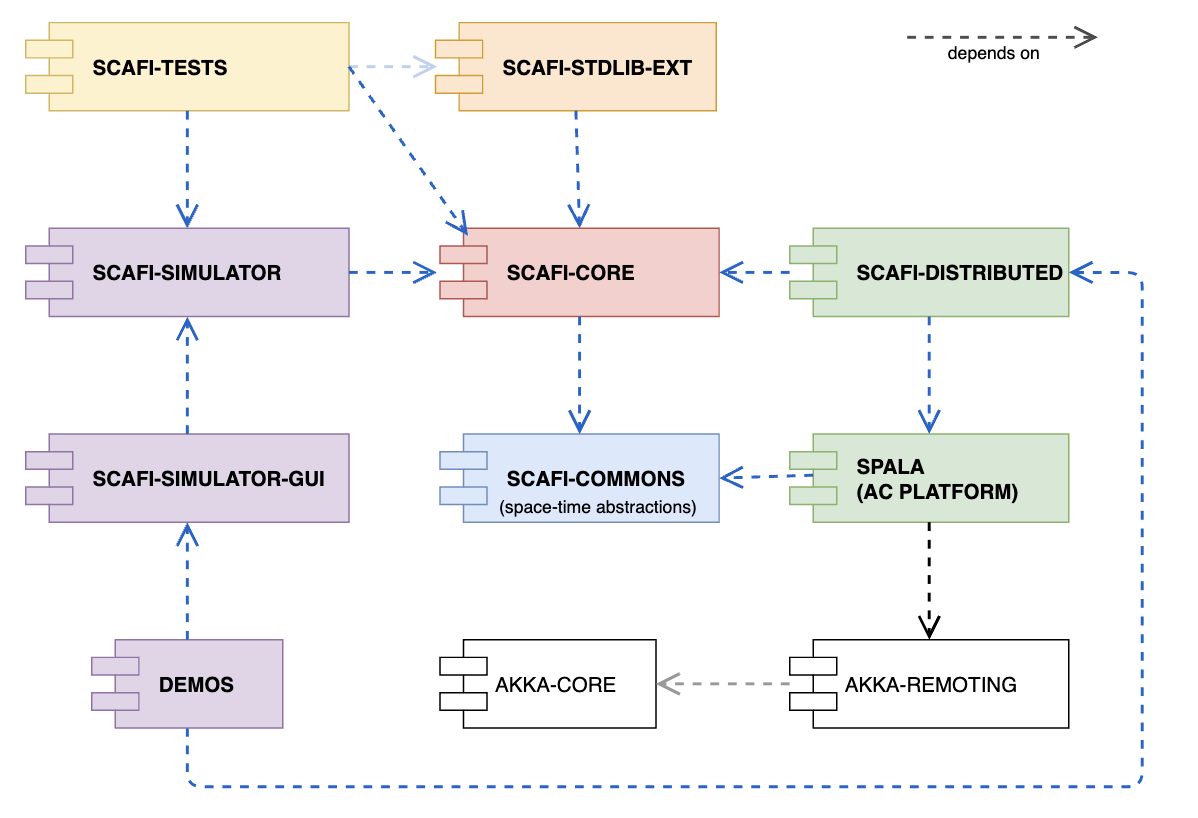
\includegraphics[width=0.7\textwidth]{figures/scafi-architecture.png}
    \caption{The ScaFi Architecture}
    \label{fig:scafi-architecture}
\end{figure}

\begin{itemize}
    \item \textbf{scafi-commons}: provides basic abstractions and utilities such as temporal and spatial abstractions;
    \item \textbf{scafi-core}: provides the aggregate programming DSL, consisting of syntax, semantics and a virtual machine together with a standard library of functions;
    \item \textbf{scafi-stlib-ext}: provides extra functionalities that require external dependencies and hence are kept separate from the core;
    \item \textbf{scafi-simulator}: provides a basic support for simulating aggregate systems;
    \item \textbf{scafi-simulator-gui}: provides a graphical user interface for the simulator;
    \item \textbf{spala}: provides an actor-based aggregate computing middleware based on the Akka framework;
    \item \textbf{scafi-distributed}: provides an integration layer between Scafi and spala;
\end{itemize}

In particular, this thesis follows up on a project that will be later introduced which took inspiration from a subset of the scafi-core module.

\section{The Rust Programming Language}
The Rust Programming Language\cite{002} is a multi-paradigm, general-purpose programming language designed originally for systems-level development. It strives to achieve both execution
speed and memory safety and efficiency while providing zero-cost abstractions and high-level features that are unusual for low-level programming languages such as C or C++.
In this section, we will go through Rust's main features and asses whether this language is suitable to develop an \acs{ac} implementation that can run on thin devices or not.

\subsection{Rust's Basic Features}
\subsubsection{Variables and mutability}
Like the majority of today's programming languages, Rust supports storing values inside variables for referencing them in various sections of the program. \\
The developer can store a value inside a variable through a \textit{let} statement:

\begin{lstlisting}[language=Rust]
    let x = 5;
\end{lstlisting}

In Rust, even if it is a statically typed language, the type of the variable can be omitted thanks to the type inference mechanism. This means that the compiler can figure out the type of the variable by looking at the value assigned to it. In this case, the type of \textit{x} is \textit{i32}, which is a 32-bit signed integer. \\

Another important feature of Rust variables is that they are immutable by default. This means that once a value is assigned to a variable, it cannot be changed.
For example, the following code will not compile:

\begin{lstlisting}[language=Rust]
    let x = 5;
    x = 6; // error: cannot assign twice to immutable variable `x`
\end{lstlisting}

Instead, the developer can opt out of the mutability by using the \textit{mut} keyword:

\begin{lstlisting}[language=Rust]
    let mut x = 5;
    x = 6; // this code compiles
\end{lstlisting}

\subsubsection{Data Types}
The Rust language supports a wide range of data types that can be both found in low-level programs and in high-level designs. These data types can be divided into two main categories: scalar types and compound types.
For scalar types, the following are supported:
\begin{itemize}
    \item \textbf{Integers}: both signed and unsigned integers of different sizes. In particular, rust supports 8, 16, 32, 64, and 128-bit signed and unsigned integers;
    \item \textbf{Floating-point numbers}: both 32 and 64-bit floating-point numbers;
    \item \textbf{Booleans}: a boolean type that can be either \textit{true} or \textit{false};
    \item \textbf{Characters}: the language's most primitive alphabetic type, represented by a single Unicode scalar value.
\end{itemize}

For compound types, the following are supported:
\begin{itemize}
    \item \textbf{Tuples}: the simplest form of product type in Rust, represented by a collection of values of possibly different types;
    \item \textbf{Arrays}: a collection of values of the same type. Unlike other languages, Rust arrays have a fixed length.
\end{itemize}

In addition to these compound types, Rust offers several other collections; for example:

\begin{itemize}
    \item \textbf{Vectors}: a collection of values of the same type. Unlike the arrays, Rust vectors have a dynamic length;
    \item \textbf{Strings}: a growable UTF-8 encoded string type;
    \item \textbf{Hash Maps}: a collection of key-value pairs, implemented as a hash table.
\end{itemize}


\subsection{The Ownership System}
Rust's Ownership System is its most unique feature and is a core part of how the language achieves memory safety without the need for a garbage collector.
The term \textit{ownership} refers to a set of rules that govern how a program's memory is managed and it is enforced by the compiler, meaning that if
a program violates them, it won't compile. This means that none of these features will cause runtime overhead for the program.

\subsubsection{Ownership Rules}
The Rust's ownership rules are the following:

\begin{enumerate}
    \item Each value in Rust has an owner.
    \item There can only be one owner at a time.
    \item When the owner goes out of scope, the value will be dropped.
\end{enumerate}

This means that a variable's validity (and presence in memory) is tied to the scope of the variable's owner: when the owner's scope is over, the compiler will automatically
call the drop function on every owned variable, freeing the memory associated with it and making it so that the variable is no longer valid.

\subsubsection{Moving and Copying}
The ownership system has implications on what happens when a variable of a certain type is copied. For example in the following code:

\begin{lstlisting}[language=Rust]
    let x = 5;
    let y = x;
\end{lstlisting}

The value of \textit{x} is copied into \textit{y}. This means that there are now two variables on the stack both with the value of 5. This is possible because x is an integer-type variable,
and integers have a fixed and known size at compile time, so they can be pushed cheaply onto the stack.

However, if we analyze the following code:

\begin{lstlisting}[language=Rust]
    let s1 = String::from("hello");
    let s2 = s1;
\end{lstlisting}

Since s1 is a String type, which does not have a known size at compile time, s1 will consist of a pointer in the stack, pointing to a heap-allocated memory that contains the actual string data, as shown in the \cref{fig:string-memory-rep}.

\begin{figure}[h]
    \centering
    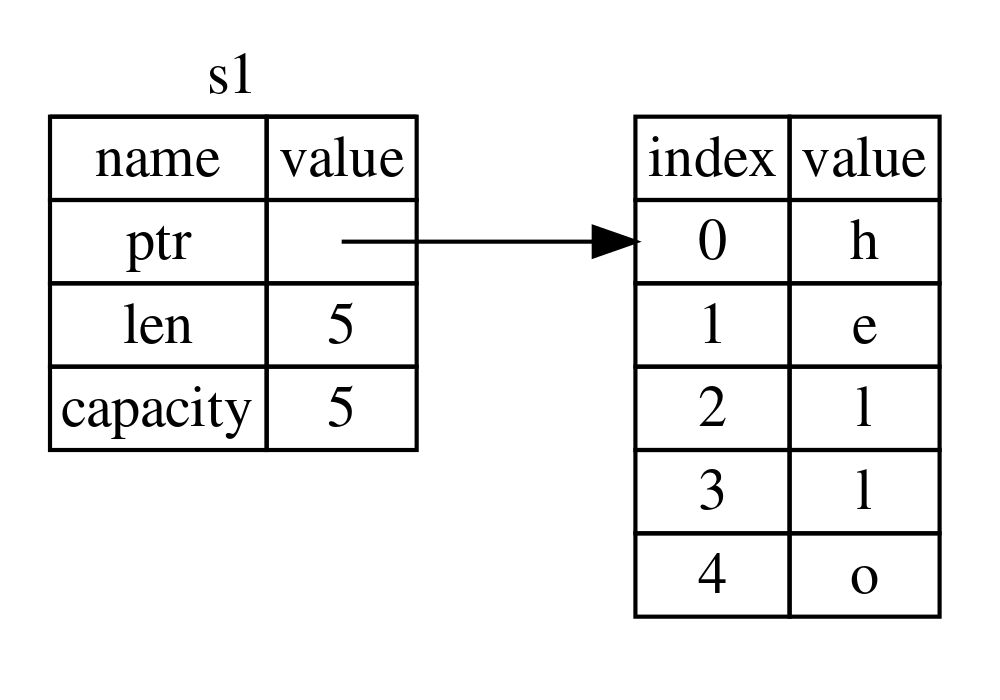
\includegraphics[width=0.5\textwidth]{figures/string-memory-rep.png}
    \caption{Representation of the memory layout of a string in Rust}
    \label{fig:string-memory-rep}
\end{figure}

When s1 gets copied into s2, only the pointer in the stack is copied, so that the memory layout of the program will look like the one in \cref{fig:string-memory-rep2}.

\begin{figure}[h]
    \centering
    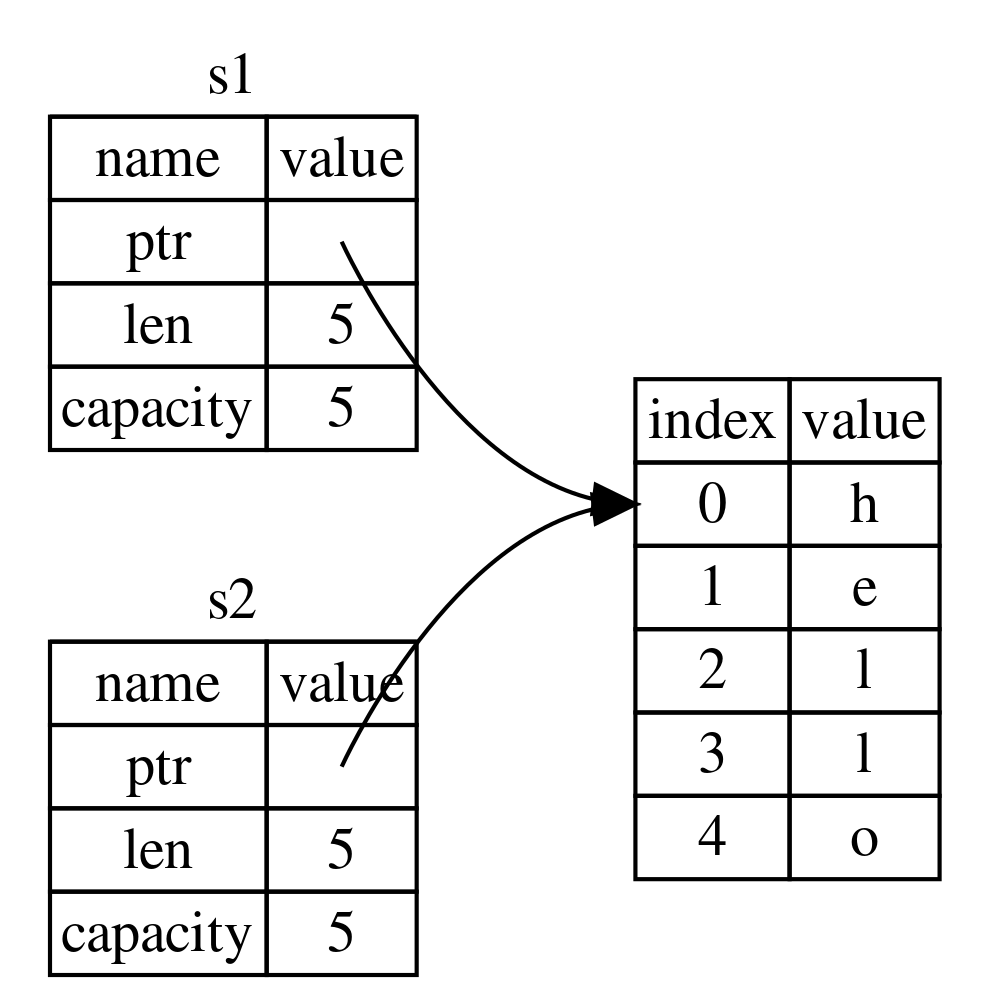
\includegraphics[width=0.5\textwidth]{figures/string-memory-rep-2.png}
    \caption{Representation of the memory layout of a string in Rust after the copy}
    \label{fig:string-memory-rep2}
\end{figure}

According to the ownership rules, when s1 and s2 go out of scope, one may think that the memory will be freed twice, causing a double-free error. However, in reality, after the copy, the compiler
will not consider s1 to be valid anymore, so when s1 goes out of scope, the memory will be freed only once, as shown in \cref{fig:string-memory-rep3}.

\begin{figure}[h]
    \centering
    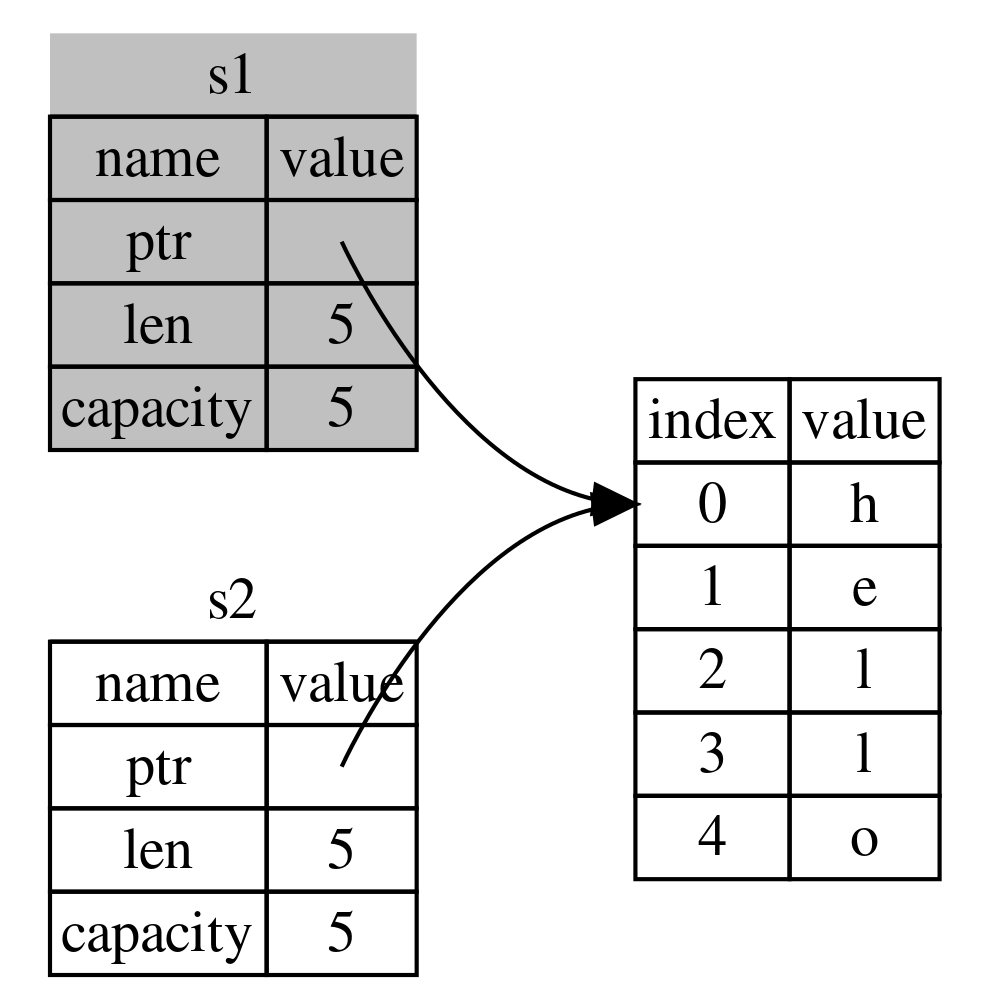
\includegraphics[width=0.5\textwidth]{figures/string-memory-rep-3.png}
    \caption{Representation of the memory layout of a string in Rust after the copy and the end of the scope of s1}
    \label{fig:string-memory-rep3}
\end{figure}

In this case, it is said that the variable s1 has been \textit{moved} into s2. This means that s1 is no longer valid and cannot be used anymore.
This happens because, by default, Rust does not create deep copies of variables of types that don't have a known size at compile time. After all, creating a deep copy of such
a variable would cause the allocation of a new memory block on the heap, an expensive operation both in terms of execution time and memory usage. If the developer
needs to create deep copies of variables stored in the heap, they can explicitly use the \textit{clone} method, which will create a new memory block on the heap and copy the data into it.

\subsubsection{Ownership and Functions}
Similarly to what happens during the variable assignment, passing a variable to a function will cause it, depending on its type, to be moved or copied, as shown in the listing \ref{lst:func_own_1}.

\lstinputlisting[language=Rust, label={lst:func_own_1}]{listings/function_ownership_ex1.rs}

Returning values from functions will also cause ownership to be transferred, as shown in the listing \ref{lst:func_own_2}.

\lstinputlisting[language=Rust, label={lst:func_own_2}]{listings/function_ownership_ex2.rs}

\subsubsection{References and Borrowing}
Instead of taking ownership of a variable and then returning it to the caller, it is possible to pass a reference to the variable to the function, so that the function can use the variable without taking ownership of it.
For a function to take a reference to a variable, it is sufficient to prefix the type definition of the variable with an ampersand (\&).
By default, references are immutable, meaning that the function cannot modify the value of the variable. If the function needs to modify the value of the variable, it is possible to take a mutable reference to it by using the \&mut keyword.

\subsection{Functional Features of Rust}
In this subsection, we will discuss some of the \ac{fp}-adjacent features of Rust.

\subsubsection{Product Types}
In FP, product types are types that combine n values of possibly different types. In Rust, it is possible to define Product types by using the \textit{struct} keyword. In particular, one can define a product type in two ways as shown in the listing \ref{lst:product_types}.

\lstinputlisting[language=Rust, label={lst:product_types}]{listings/product_types.rs}

It is also possible to add functionality to the ADTs created by using the \textit{impl} keyword, as shown in the listing \ref{lst:product_types_impl}.

\lstinputlisting[language=Rust, label={lst:product_types_impl}]{listings/product_types_impl.rs}

\subsubsection{Sum Types and Pattern Matching}
In FP, a sum type represents a choice between some types. In Rust, we can define Sum types by using the \textit{enum} keyword. It is also possible to perform pattern matching over a sum type, as it is shown in the listing \ref{lst:sum_types}.

\lstinputlisting[language=Rust, label={lst:sum_types}]{listings/sum_types.rs}

\subsubsection{Polymorphism}
Rust supports polymorphism through traits. Rust's traits are similar to Haskell's typeclasses and they allow us to define a particular functionality that a particular type has.
For example, we can implement Haskell's Show typeclass in Rust as shown in the listing \ref{lst:polymorphism}.

\lstinputlisting[language=Rust, label={lst:polymorphism}]{listings/polymorphism.rs}

\subsubsection{Lambdas and Closures}
In FP, lambda functions or anonymous functions, are functions that are not bound to a name. Moreover, closures are lambda functions that can ``capture'' the environment in which they are defined.
In Rust, both lambdas and closures are supported, though they are both called closures. Like in other languages, Rust closures can be assigned to variables and passed to functions.
When defining a closure in Rust, it is important to reason about the ownership of the variables that are captured by it. The listing \ref{lst:closures} shows some examples of closures in Rust.

\lstinputlisting[language=Rust, label={lst:closures}]{listings/closures.rs}

\subsubsection{Iterators}
The Iterator pattern allows to traverse collection of elements in a particular manner, performing some task on each element in turn. The iterator is responsible for the traversal logic
so that the developer does not need to reimplement it each time. In Rust, the Iterator pattern is implemented through the \textit{Iterator} trait, which is implemented by the standard library's collections:

\begin{lstlisting}[language=Rust]
    trait Iterator {
        type Item;
        fn next(&mut self) -> Option<Self::Item>;
        //Other default methods omitted
    }
\end{lstlisting}

The developer can also implement the Iterator trait for his custom types, enabling many functionalities that are divided into the following categories:

\begin{itemize}
    \item \textbf{Consumer Adaptors}: these are methods that take ownership of the iterator because they traverse it using its next method, thus consuming it. Examples of consumer adaptors are reducing methods like \textit{sum};
    \item \textbf{Iterator Adaptors}: these are methods that don't take ownership of the iterator, since they take an iterator and return another, modified one. An example of an iterator adaptor is the \textit{map} method, which applies a function to each element of the iterator;
\end{itemize}

\subsubsection{Error Handling}
Rust provides mechanisms for error handling that are equivalent of the ones we can find in most of the modern functional programming languages: Options and Results.
The Option type models a value that can be absent and is implemented through an enum that can have two variants: Some, which contains a value, and None, which represents the absence of the value.
This type offers many functions to manipulate its hypotetical value, such as \textit{map}, \textit{for\_each} and \textit{unwrap}, which attempts to get the value of the enum if present, panicking (the Rust
equivalent of throwing an exception) if the value is not present.
Another common mechanism for error handling in rust is the Result type, which represents a computation that may fail. This type is similar to the ``Either'' type of some functional languages like Haskell or Scala,
and it is also implemented with an enum that can have two variants: Ok, which contains a value, and Err, which contains an error value. This type also offers many functions to operate with it, such as
\textit{unwrap}, \textit{unwrap\_or}, \textit{map} and \textit{map\_err}.
Since both of these types are enums, it is possible to deconstruct them via pattern matching.

\subsection{Metaprogramming in Rust}
In computer science, \textit{metaprogramming} is the technique by which a programmer can write code that generates or manipulates other code. In Rust, this technique is enabled
by its powerful \textit{macro} system. There are two main families of macros in Rust: declarative macros and procedural macros.

\subsubsection{Declarative Macros}
Declarative macros are the most common type of macros in Rust. They are invoked similarly to functions, however, they can have a variable number of arguments and can be called with different types of parenthesis.
At their core, declarative macros are similar to match expressions, but instead of matching against a value, they match against the Rust code that is passed to the macro, which can also include but it's not limited to expressions.
The listing \ref{lst:declarative_macros} shows an example of a declarative macro that implements the \textit{vec!} macro.

\lstinputlisting[language=Rust, label={lst:declarative_macros}]{listings/declarative_macros.rs}

This thesis will not introduce the reader to procedural macros, as they constitute a deeply technical topic that is not relevant to the scope of this work.

\subsection{Why Rust}
As shown in the previous sections, Rust is a general-purpose programming language designed with a focus on safety, speed and efficiency. These design principles, coupled with high-level features
more adjacent to functional programming than to low-level programming, making Rust a good candidate for developing \ac{ac} implementations that can run on thin devices.


\section{Towards a Rust-based AC Implementation: the RustFields Project}
The RustFields Project\cite{001} was an attempt to bring \ac{ac} to thin devices exploiting the Rust programming language. The project aimed to reach its goals by developing two lines of research:
\begin{itemize}
    \item A pure, Rust-based implementation of AC in the same vein as the ScaFi framework;
    \item A mixed approach that aims to mix ScaFi's highly expressive API with Rust's performance and efficiency;
\end{itemize}

\subsection{RustFields Architecture}
As stated in the official documentation of the project: \\
``    Since the project was meant as an exploration of different options for bringing aggregate programming into native contexts, we decided to explore both solutions. The resulting architecture reflects this choice: in fact, we decided to develop a standalone aggregate programming framework in the Rust language, while also experimenting with different ways to integrate it with the Scala ScaFi’s ecosystem.
''

The resulting architecture reflects this choice and this is made evident in the diagram in \cref{fig:rustfields-architecture}.

\begin{figure}[h]
    \centering
    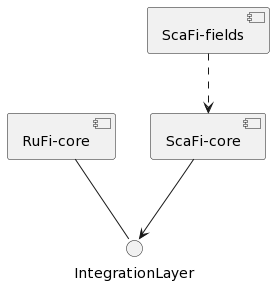
\includegraphics[width=0.5\textwidth]{figures/diagrams/img/rustfields-full-architecture.png}
    \caption{The RustFields Architecture}
    \label{fig:rustfields-architecture}
\end{figure}

In the architecture diagram shown in \cref{fig:rustfields-architecture}, the RuFi-core is responsible for implementing in Rust the core concepts of the new \ac{ac} implementation,
structured in a way that is somewhat similar to the ScaFi's core. Then, an \textit{integration layer} was built on top of the Rust core to allow communication
between Scala and Rust code. From then, the project development was divided into two main branches:
\begin{itemize}
    \item The expansion of the RuFi core, which aimed to serve as a base for a fully-fledged \ac{ac} implementation in Rust;
    \item The development of the integration layer, aimed to bring the best of both worlds by allowing the developer to use the expressive API of ScaFi with the performance and efficiency of Rust.
\end{itemize}

The design of the RuFi-core component is of particular interest since this thesis aims to expand it and further develop an \ac{ac} implementation in Rust, and it will be discussed
later in the Chapter \ref{chap:design}.